\chapter{Equal information, different topology}\label{ch:separation}

Does counting histories, or counting them together with their local neighbourhoods, tell an observer whether the history space has a hole? The answer has four layers. (i) \emph{In general no}: there are information-equivalent, topologically inequivalent pieces at every radius $\le2$ (\cref{sec:witnesses}). (ii) \emph{In the two anchor families} the history count alone suffices, because it is injective on the comparable window (\cref{sec:window}). (iii) \emph{On the six-label census} the count alone does not suffice, but radius-two histograms do, with zero residual entropy (\cref{sec:census-entropy}). (iv) That zero is a statement about collisions in a finite sample, not about prediction; \cref{sec:predictive} separates descriptive from predictive information and preserves the two predictions that failed.

\section{Information-equivalent, topologically inequivalent pieces}\label{sec:witnesses}
By a \emph{piece} we mean a content with a source whose admissible set is a single component. Two pieces are \emph{information-equivalent at radius $r$} if they have the same number of histories, the same class sizes and the same multiset of ball sizes $|B_i(w)|$ for $i\le r$.
\begin{proposition}[information-equivalent, topologically inequivalent pieces; computer-assisted]\label[proposition]{prop:witnesses}
There are pairs of arithmetic pieces with equal $N$, equal class structure (hence equal Hartley entropy $\log_2N$ and equal class entropies), agreeing in the fine signature through radius $s-1$ and differing in Betti vectors; $s$ is the \emph{separating radius}:
\begin{center}\footnotesize\setlength{\tabcolsep}{3pt}
\begin{tabular}{@{}llllcl@{}}\toprule
ID & piece A (content @ source) & $\beta(A)$ & piece B & $\beta(B)$ & $s$ and what differs\\ \midrule
W1 & $\{2,3,14,15\}@210$ & $(1,1,0,0)$ & $\{1,2,3,4\}@6$ & $(1,0,0,0)$ & $1$: $E=20$ vs $21$\\
W2 & $\{2,3,8,9\}@72$ & $(1,1,0,0)$ & $\{2,3,5,6\}@30$ & $(1,0,0,0)$ & $1$: $E=20$ vs $21$\\
W3 & $\{2,3,8,9,14\}@1008$ & $(1,0,1,0,0)$ & $\{1,2,3,5,7\}@105$ & $(1,0,0,0,0)$ & $2$: squares $66$ vs $60$\\
W4 & $\{2,3,8,9,10\}@72$ & $(1,1,0,0,0)$ & $\{1,2,3,5,9\}@18$ & $(1,0,0,0,0)$ & $2$: squares $21$ vs $19$\\
W5 & $\{2,3,9,15,21\}@189$ & $(1,1,0,0,0)$ & $\{1,2,12,13,26\}@52$ & $(1,0,0,0,0)$ & $3$: hexagons $1$ vs $2$\\
W6 & $\{2,3,8,21,26\}@273$ & $(2,1,0,0,0)$ & $\{6,8,9,14,15\}@168$ & $(2,0,0,0,0)$ & $3$: hexagons $0$ vs $1$\\ \bottomrule
\end{tabular}
\end{center}
with $N=16,16,96,40,24,18$ histories respectively. In W5 and W6 the two pieces have equal $N$, $E$ (32 and 17), square count ($7$; none) and equal fine statistics through radius $2$; their Betti numbers differ by exactly one hexagonal $2$-cell, which no statistic of radius $\le2$ sees. The Euler characteristic $\sum(-1)^if_i=\sum(-1)^i\beta_i$ holds on every row.
Consequently: histories-counting ($r=0$), one-swap ($r\le1$) and two-swap ($r\le2$) accessibility do not detect history homology on arithmetic pieces.

\end{proposition}
Witnesses W5 and W6 are the sharpest: radius-two data determine $N$, $E$ and $Q$ and the identity of \cref{thm:radius2} contains no hexagon term, yet these pieces differ by one hexagonal face. The combinatorial source of the difficulty is \cref{prop:petrie}: a hexagon bounding a braid face and a six-cycle bounding none cannot be told apart by the graph alone without the cube-product property.
For distinct-label pieces the fine signature through radius $3$ determines the permutohedral Betti vector in every case examined ($k=4$ with labels $\le70$, $k=5$ with labels $\le26$); whether radius three suffices in general is unknown, and radius two provably fails.

\section{The comparable window: where the count suffices}\label{sec:window}
Return to the anchors of \cref{ch:topology}: $\lambda_A=(2,3,4,5,8,9)$ with $m_0=288$ and $\lambda_B=(2,3,6,7,8,9)$ with $m_0=432$. The sources $m=m_0t$ with $t\in\{1,\dots,60\}$ realise only eight of the finite lattice of systems (\cref{prop:finite-lattice}). Let $Y_{\mathrm{anc}}$ be the anchored hole state of \cref{ch:access}.
\begin{observation}[exact survival entropy and recovery on the window; finite-exact]\label[observation]{obs:anchored}
Under the uniform measure on $t=1,\dots,60$:
\begin{enumerate}[label=(\roman*)]
\item $Y_{\mathrm{anc}}=1$ exactly for $\gcd(t,30)=1$ ($16/60$; $p=4/15$) for $\lambda_A$ and for $\gcd(t,42)=1$ ($17/60$) for $\lambda_B$ (\cref{thm:anchor}); $H(Y)=-p\log_2p-(1-p)\log_2(1-p)=0.83664$ bits for $\lambda_A$ and $0.85995$ bits for $\lambda_B$.
\item The eight system classes on the window have eight \emph{distinct} history counts: $372,408,444,480,612,648,684,720$ ($\lambda_A$) and $276,312,324,360,612,648,684,720$ ($\lambda_B$) --- recomputed from the admissibility rule. Therefore $H(Y\mid N)=0$: on the comparable window the history count alone recovers the hole state, and so do all finer levels. There is no pair of sources on the window with equal history count and different hole state.
\item Beyond the window, over all system classes, $\lambda_A$ has no binary separating pair at any level. $\lambda_B$ has exactly one at the level of the count: $m=648$ ($N=276$, state $\mathrm{NA}$) and $m=432$ ($N=276$, state $1$); it is separated by the ball histograms. This is not a ``filled vs survives'' pair: $648$ is not a multiple of $432$, so $Y_{\mathrm{anc}}(648)$ is undefined and counted as $0$ only by the binary convention.
\item \emph{Arrow law.} On the window, multiplying the source by a prime of the modulus ($2,3,5$ for $\lambda_A$; $2,3,7$ for $\lambda_B$) sends $Y=1\mapsto0$ at once, and $Y=0$ stays $0$: the filled state is absorbing (for divisibility $m\to mp$, not for time). The exact information jump from the surviving source is, for $\lambda_A$, $\log_2(408/372),\log_2(444/372),\log_2(612/372)=0.1333,0.2553,0.7182$ bits for $\times2,\times3,\times5$, and for $\lambda_B$ $\log_2(312/276),\log_2(324/276),\log_2(612/276)=0.1769,0.2313,1.1489$ bits for $\times2,\times3,\times7$. Multiplication beyond the cap leaves $A$, $N$ and $Y$ unchanged.
\end{enumerate}

\end{observation}
For $\lambda_A$ the counting law is $N(288t)=372+36[2\mid t]+72[3\mid t]+240[5\mid t]$, an injective function of the triple of indicators on the window because the increments $36,72,240$ have distinct subset sums. This is a numerical coincidence of the family rather than a mechanism; for $\lambda_B$ the non-additive $3\cdot7$ interaction ($+24$) does not destroy injectivity.

\section{The census: the count does not suffice, radius two does}\label{sec:census-entropy}
Let $\mathcal D$ be the six-label census: $8{,}008$ contents with labels in $\{1,\dots,16\}$ and $346{,}859$ regimes (distinct nonempty admissibility sets). Let $Y=\mathbf 1[\beta_2(K_A;\F)>0]$.
\begin{observation}[the count does not determine $Y$ on the census; finite-exact]\label[observation]{obs:equal-N}
The recomputation of every Betti vector with a second engine gives $158$ regimes with $\beta_2>0$ ($157$ with $\beta_2=1$, one with $\beta_2=3$), identical as a set to the list of \cref{obs:census-H2}. The $158$ positives take $59$ distinct values of $N$ (ranging over $1\ldots720$). There are $326{,}912$ (positive, negative) pairs with equal $N$; $72$ of them lie in the same content, and $51$ positives have a same-content negative partner. Every one of the $158$ positives has at least one negative with equal $N$. Hence $H(Y\mid N)>0$ under each of the ensembles below.

\end{observation}
\begin{example}[a certified pair with equal count; finite-exact]\label[example]{ex:pair}
Content $(2,3,4,5,8,15)$ at sources $480$ and $800$: both have $N=396$ (re-derived by simulating divisibility), but $f$-vectors $(396,900,669,173,10,0)$ and $(396,882,636,156,7,0)$ and Betti vectors $(1,0,1,0,0,0)$ and $(1,0,0,0,0,0)$; the positive carries an explicit $2$-cycle and $2$-cocycle with $\varphi(z)=1$ (\cref{lem:certificate}), the negative has $\beta_2=0$ by two independent GF(2) rank routes. The smallest exhibit with equal radius-one data is content $(2,4,5,9,14,15)$ at $2520$ ($\beta_2=1$) and $3780$ ($\beta_2=0$): both have $N=540$, equal $h_1$, equal square count $Q=738$, equal $E=1278$, equal $S_{d2}=12212$ and equal $S_B=9800$, but $S_{BB}=180420$ vs $180408$ (different $h_2$); their $f$-vectors differ in $f_3$ only ($291$ vs $292$). They share $468$ of $540$ arrangements.

\end{example}
\begin{figure}[ht]\centering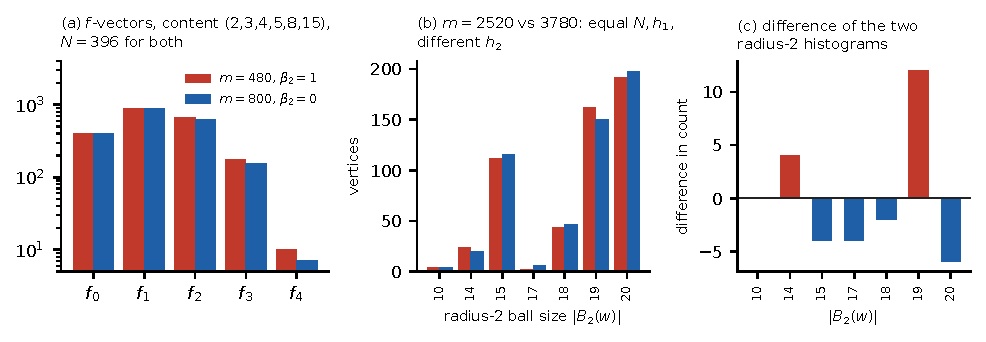
\includegraphics[width=\textwidth]{figures/fig_equal_N.pdf}
\caption{Equal history count, different topology. (a)~$f$-vectors of the pair of \cref{ex:pair} with $N=396$: the surviving hole (red) has more cells than the filled complex (blue) in every dimension $\ge1$. (b,c)~Radius-two ball-size histograms of the pair $2520$ and $3780$ at $N=540$, which have equal radius-one data; the histograms differ at a few vertices only. All values are recomputed exactly.}\label{fig:equal-N}
\end{figure}
\begin{theorem}[no function of the radius-one data and the square-incidence data determines $Y$; computer-assisted]\label[theorem]{thm:no-radius1}
There is no function of $(N,h_1,h_q)$ --- hence none of $(N,E,Q,S_{d2},S_B)$ --- whose value determines $Y$ on $\mathcal D$. Indeed there are $165$ (positive, negative) pairs with the same $(N,h_1,h_q)$, involving $22$ positives, and all have different $h_2$; the pair of \cref{ex:pair} is one.

\end{theorem}
\begin{table}[ht]\centering\footnotesize\setlength{\tabcolsep}{3pt}
\begin{tabular}{@{}lrrrrrrrr@{}}\toprule
ensemble & size & $H(Y)$ & $H(Y|N)$ & $H(Y|N,f_1)$ & $H(Y|N,\chi)$ & $H(Y|N,h_1)$ & $H(Y|f)$ & $H(Y|N,h_2)$\\ \midrule
$\mathcal E_{\mathrm{all}}$ & $346{,}859$ & $.005713$ & $.004467$ & $.002172$ & $.000109$ & $.000619$ & $0$ & $0$\\
$\mathcal E_{\mathrm{band}}$ & $93{,}018$ & $.018078$ & $.016659$ & $.008100$ & $.000406$ & $.002309$ & $0$ & $0$\\
$\mathcal E_{\mathrm{rank}}$ & $219{,}146$ & $.008231$ & $.006276$ & $.003140$ & $.000168$ & $.000803$ & $0$ & $0$\\ \bottomrule
\end{tabular}
\caption{Exact residual entropy (bits) of $Y=\mathbf 1[\beta_2>0]$ given observations, for three uniform ensembles on the census. $\mathcal E_{\mathrm{band}}$: regimes whose $N$ is attained by a positive regime. $\mathcal E_{\mathrm{rank}}$: one regime per distinct rank-indexed family mask. $f$ denotes the full $f$-vector. Plug-in values, in-sample (\cref{sec:predictive}).}\label{tab:residual}
\end{table}
\begin{observation}[radius-two data recover $Y$ on the census; the zero is a collision statement; finite-exact, bounded in scope]\label[observation]{obs:residual}
On $\mathcal D$ the observation $O_h=(N,h_1,h_2)$ has zero mixed classes in all three ensembles ($8{,}208$ classes in $\mathcal E_{\mathrm{all}}$, none mixed), so $H(Y\mid O_h)=H(Y\mid O_G)=H(Y\mid O_A)=0$ (\cref{thm:obs-ladder}). The separation $H(Y\mid N)>0$ therefore does \emph{not} persist once radius-two accessibility is added. Of partial observables, $(N,h_2)$ and the full $f$-vector already give $0$, while $(N,h_1)$, $(N,f_1)$, $(N,\chi)$ leave $66$, $151$, $8$ positives sharing their signature with a negative.
These are empirical facts about $\mathcal D$ ($\le16$ labels, six distinct labels). They are not theorems, they do not extend to other label ranges or sizes, and their arithmetic origin is \textbf{open}. Moreover the zero residual is a statement about \emph{collisions} of signature classes in a finite census; it is not a statement about information that generalises (\cref{sec:predictive}).

\end{observation}
Two quantities are in play. The \emph{Hartley} ambiguity $\log_2N$ of a regime measures the multiplicity of its histories; the \emph{Shannon} residual $H(Y\mid\cdot)$ measures what a given observation leaves unknown about topology. They are unrelated in general: \cref{prop:witnesses} and \cref{obs:equal-N} exhibit equal Hartley and different topology, and the zero of \cref{obs:residual} exhibits zero residual with positive Hartley. The unifying fact is the ladder of \cref{thm:obs-ladder}: every observation is a function of $A$, and topology is a function of $A$ that is not a function of the cheap observations.

\section{Descriptive versus predictive information}\label{sec:predictive}
A zero residual entropy is a statement about a \emph{finite sample of signatures}. It can arise because the signature is informative, or because it is nearly injective, so that every system sits alone in its class. This section separates \emph{descriptive} information (how well the classes of a signature split positives from negatives in a sample) from \emph{predictive} information (how much a rule learned on one sample says about topology in another), and records the two statements that did not survive testing.

Let $\mathcal S$ be a finite set of systems, $Y=\mathbf 1[\beta_2>0]$ and $O$ an observation. A \emph{class} is a fibre of $O$, \emph{mixed} if it contains both values of $Y$. The \emph{plug-in} conditional entropy is computed from empirical class frequencies,
\[
H_{\mathrm{plug}}(Y\mid O)=\sum_{c}\frac{|c|}{|\mathcal S|}\,\mathrm h\!\left(\frac{|c\cap Y^{-1}(1)|}{|c|}\right),\qquad \mathrm h(p)=-p\log_2p-(1-p)\log_2(1-p).
\]
Two ensembles are used: the \emph{natural} ensemble, uniform on regimes (positives are rare, $H(Y)=0.005713$ bits on the census), and the \emph{balanced} ensemble, which weights positives and negatives equally. Both are experimental conventions, not probability laws of the grammar.
\begin{lemma}[a zero is cheap when signatures are fine; analytic]\label[lemma]{lem:zero-cheap}
$H_{\mathrm{plug}}(Y\mid O)=0$ iff $O$ has no mixed class on $\mathcal S$. In particular, if $O$ is injective on $\mathcal S$ then $H_{\mathrm{plug}}(Y\mid O)=0$ for \emph{every} target $Y$. A zero residual therefore certifies information about $Y$ only relative to a null model that has the same class sizes.
\end{lemma}
\begin{proof}
A class contributes $\mathrm h(p)$, which vanishes iff $p\in\{0,1\}$ iff the class is pure. If $O$ is injective every class is a singleton.
\end{proof}
\begin{observation}[smallest separating signatures on the census; finite-exact]\label[observation]{obs:separators}
(a) No single scalar from the pool has zero residual; the best, $S_{BB}$, hides $36$ positives in $18$ mixed classes.
(b) The minimal separating \emph{pairs} include $(N,S_{BB})$, $(Q,S_{BB})$, $(S_B,S_{BB})$ and, in the second-order pool, $(Q,S_{s2})$, $(S_{d2},S_{s2})$, $(S_{d3},S_{s2})$, $(S_{q2},S_{s2})$, $(S_{s2},S_{ds})$, $(S_{s2},S_{dq})$, $(S_{s2},S_{sq})$. Every separating pair contains a second-order radius-two sum ($S_{BB}$ or $S_{s2}$). The full histogram $h_2$ and the $f$-vector also give zero residual.
(c) Of the $66$ positives left in mixed classes by $(N,h_1)$, adding \emph{one} scalar resolves: $S_{s2}$: all $66$; $S_{BB}$: all $66$; $f_3$: $64$; $S_{ds}$ and $S_{sq}$: $59$; $h_x$: $47$; $S_{q2},S_{dq}$: $44$; $Q$: $42$; $S_B$: $42$; nothing of first order ($E,S_{d2},S_{d3},d_{\max},d_{\min}$) resolves any.
(d) Non-triviality: for $(N,S_{BB})$ and the other separating pairs, $104$ of the $151$ positive masks lie in pure classes of size $\ge2$ (the largest pure positive class has $15$ members); placing the positives at random among regimes of equal $N$ hides $133$--$149$ of the $151$ (mean $143$) in mixed classes, and none of $300$ shuffles gave $0$. Forty-seven positives are alone in their class.

\end{observation}

\subsection*{A pre-registered test}
The signatures $S_A=(N,S_{BB})$, $S_B=(Q,S_{s2})$ and $S_C=(S_{d2},S_{s2})$ were found on the census to have no mixed class. Before any held-out system was generated, the following was fixed in writing, together with sampling frame, random seeds and a hash of the feature file. A held-out set H6 of $6000$ contents was drawn uniformly from six-subsets of $\{1,\dots,22\}$ whose maximum label lies in $17$--$22$, with all regimes of each content. Prediction P1 was that each of $S_A,S_B,S_C$ has no mixed class in H6 or in the pooled set, and could be falsified by a single mixed class; P2 was that $(N,h_1)$ leaves some positive in a mixed class. An exploratory seven-label sample H7 of $120$ contents carried no prediction.
\begin{observation}[outcome of the pre-registered held-out test; bounded]\label[observation]{obs:preregistered}
H6 contains $263{,}124$ regimes, $132$ positives; pooled with $\mathcal D$: $609{,}983$ regimes, $290$ positives.
\begin{itemize}[nosep]
\item $S_B=(Q,S_{s2})$: $0$ mixed classes in H6 and pooled. \textbf{Confirmed.}
\item $S_C=(S_{d2},S_{s2})$: $0$ mixed classes in H6 and pooled. \textbf{Confirmed.}
\item $(N,h_1,h_2)$ (not a registered prediction): $0$ mixed classes in H6 and pooled.
\item $S_A=(N,S_{BB})$: $3$ mixed classes ($3$ positives) in H6 and $6$ mixed classes ($10$ positives) pooled. \textbf{The pre-registered prediction for $S_A$ is falsified.} In $5$ of the $6$ classes the colliding systems differ in $Q$ and $S_{s2}$; in the sixth ($N=576$) they differ in $S_{s2}$ only.
\item P2: $(N,h_1)$ leaves $143$ of the $290$ pooled positives in mixed classes. \textbf{Confirmed.}
\end{itemize}
Consequently the pre-registered claim ``all three pairs separate'' is false as stated (P1 fails through $S_A$). The weaker, more structured statement ``$(Q,S_{s2})$, $(S_{d2},S_{s2})$ and the $h_2$ histogram separate'' survived out of sample on $263$ thousand new regimes. Non-triviality on the pooled set: $206$ of the $290$ positives lie in pure classes of size $\ge2$; the random-placement null hides $267$--$285$ of $290$; the real value is $0$. In the seven-label exploratory sample ($10{,}130$ regimes, $11$ positives) every candidate signature, including $(N,h_1)$, has zero mixed classes while $N$ alone does not: the sample is too small and its signatures nearly injective to discriminate, and no transfer claim is made at $k=7$.

\end{observation}
$(N,S_{BB})$ is a good fingerprint on $\mathcal D$ but not a law.

\subsection*{A general principle that is false}
After the test the question was whether $(Q,S_{s2})$ separates for a structural reason, such as every arithmetic system being prefix-defined, or only because of arithmetic closure.
\begin{observation}[the pair $(Q,S_{s2})$ is not sufficient in general; finite-exact and bounded]\label[observation]{obs:S2-falsified}\leavevmode
\begin{itemize}[nosep]
\item On arithmetic regimes ($\mathcal D\cup$H6, $609{,}983$ regimes, $290$ positives) there is no mixed class of $(Q,S_{s2})$, $(N,h_1,Q,S_{s2})$ or $(N,h_1,h_2)$, and every one of the $206$ positives that shares its $(Q,S_{s2})$ with another regime shares it only with positives (partner-positive rate $1.000$ against a base rate $0.0005$).
\item On \emph{prefix-family systems} (sets of orderings all of whose prefix sets lie in a family; $109{,}906$ distinct random systems, $4{,}796$ positives): $(Q,S_{s2})$ has $60$ mixed classes ($89$ positives hidden); $(N,Q,S_{s2})$ has $28$ ($52$ hidden); $(N,h_1,Q,S_{s2})$ has $24$ ($48$ hidden);\allowbreak\ $(N,h_1,Q,S_{s2},S_{ds})$\allowbreak\ has $21$ ($43$).
\item \emph{A certified counterexample.} Two prefix-family systems with $N=388$, identical $h_1$, identical square-incidence histogram, $Q=397$, $S_{s2}=85536$, equal $S_{ds}$, $S_B$ and even $S_{BB}=96888$, but $\beta_2=1$ versus $0$ (the positive with an explicit $2$-cycle and cocycle verified from the definition; the negative with $\beta_2=0$ by two rank routes and an independent engine); they differ in $h_2$ and $f_3$ ($105$ vs $106$). Neither is an arithmetic census regime.
\item The full radius-two histogram $(N,h_1,h_2)$ has zero mixed classes in all three tested classes (arithmetic $609{,}983$; prefix families $109{,}906$ with $4{,}796$ positives; arbitrary vertex sets $30{,}000$ with $11{,}373$ positives); in prefix families $2{,}991$ positives share their $(N,h_1,h_2)$ with other systems, all partners positive.
\end{itemize}
Hence the separation by $(Q,S_{s2})$ is \emph{not} a consequence of the prefix structure or of local graph combinatorics alone, and no radius-two \emph{moment} signature $(N,Q,S_{s2},S_{ds},S_B,S_{BB})$ is sufficient in general. It holds on every arithmetic regime tested. Whether arithmetic closure forces it is open. The principle ``radius-two scalar moments determine topology'' is \textbf{falsified} as a general statement.

\end{observation}
\begin{observation}[the seven hard positives; bounded]\label[observation]{obs:hard-positives}
On the census the positives left in mixed classes by $(N,h_1,S_{ds})$ number $7$ (by $(Q,S_{ds})$: $10$; by $(N,h_1,Q)$: $24$); on $\mathcal D\cup$H6 these numbers are $38,53,74$. In every one, $S_{s2}$ resolves the class, but narrowly: the positive's $S_{s2}$ is smaller than the partner's by $16$ (or $48$), relative margins of order $10^{-4}$ --- for instance content $(2,3,8,9,11,14)$ at $77$ and content $(2,3,4,8,14,15)$ at $1680$. In all $13$ mixed classes of $(N,h_1,Q,S_{ds})$ on $\mathcal D\cup$H6 the positive has the smaller $S_{s2}$ (gap $-16$ typically); in the $30$ mixed classes of $(N,h_1,Q)$ only $21$ have all positives below all negatives, so there is no one-sided inequality law. Why $S_{s2}$ --- a sum over pairs of two-step walks --- correlates with the topology is not explained; the simplest forbidden-subset motifs (dead subsets, complementary dead pairs) do not discriminate ($142/158$ positives against $1333/2000$ sampled negatives have a complementary dead pair).

\end{observation}

\subsection*{Descriptive versus predictive}
\begin{observation}[plug-in information is descriptive; finite-exact]\label[observation]{obs:plugin}
On $\mathcal D\cup$H6, balanced ensemble ($609{,}983$ systems, $290$ positives): $H(Y\mid N)=0.4552$, $H(Y\mid N,h_1)=0.0126$, $H(Y\mid N,h_1,h_q)=0.0016$ and $H(Y\mid Q,S_{s2})=H(Y\mid N,h_1,Q,S_{s2})=H(Y\mid N,h_1,h_2)=0$ bits. On the natural ensemble over $\mathcal D$: $I(Y;N)=0.00124$ of $0.00571$ bits ($21.8\%$), $I(Y;N,h_1)=0.00509$ ($89.1\%$), zero residual for $(N,h_1,Q,S_{s2})$. These plug-in values measure how little the exact signature classes overlap, and fine signatures ($55{,}000$--$110{,}000$ classes) leave most negatives alone in their class (\cref{lem:zero-cheap}). They are \emph{not} predictive information.

\end{observation}
\begin{observation}[out-of-sample information; bounded]\label[observation]{obs:oos}
Define the information \emph{gained about $Y$} by an observation as $1-$ the balanced cross-entropy of a classifier fitted on one sample and evaluated on the other (the classifier family and the exact fitting protocol are those of the original computation and are not reproduced here). Train on $\mathcal D$ and test on H6 (first number) or the reverse (second number), balanced test ensemble:
\begin{center}\small
\begin{tabular}{@{}lcc@{}}\toprule
observation & $\mathcal D\to$H6 & H6$\to\mathcal D$\\ \midrule
$N$ alone & $0.31$ & $0.38$\\
radius-one scalars & $0.28$ & $0.52$\\
radius-one $+$ square count & $0.44$ & $0.66$\\
all radius-two scalars & $0.44$ & $0.68$ (AUC $0.96$/$0.98$)\\
$(Q,S_{s2})$ alone & $0.29$ & $0.45$\\
exact-signature lookup with back-off & $-1.05$ & $-1.19$\\ \bottomrule
\end{tabular}
\end{center}
The exact lookup is worse than ignorance: $61\%$ of the held-out positives ($\mathcal D\to$H6) have a signature never seen in training. An observer learning from one sample therefore recovers at most about $0.4$--$0.7$ of the one bit about generative topology; the zero residual of exact signatures is a statement about collisions, not about generalisation.

\end{observation}
\begin{figure}[ht]\centering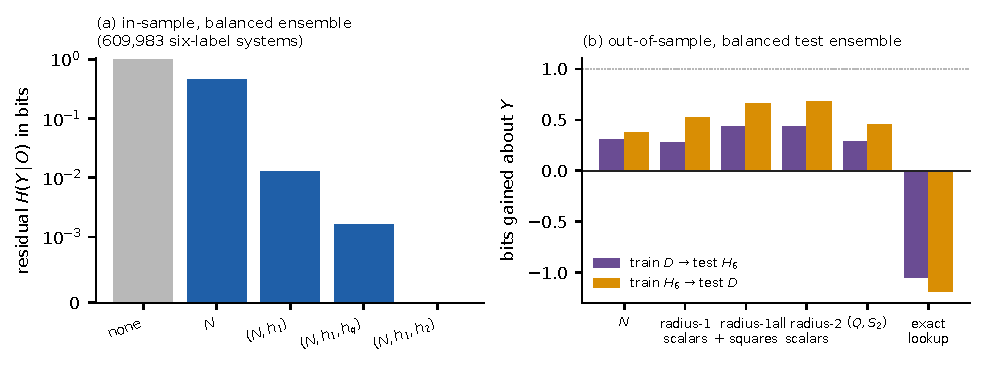
\includegraphics[width=\textwidth]{figures/fig_recovery.pdf}
\caption{(a)~In-sample residual entropy $H(Y\mid O)$ of the hole indicator by observation level, balanced ensemble on $609{,}983$ six-label systems. (b)~Information gained about $Y$ when a rule is trained on one sample and tested on the other. The in-sample residual falls to $0$ while the out-of-sample gain saturates near $0.4$--$0.7$ bits. Both panels plot values obtained in earlier computations (cf.\ \cref{app:status}); none is recomputed here.}\label{fig:recovery}
\end{figure}
\begin{observation}[like-for-like replication for the first Betti number; finite-exact]\label[observation]{obs:beta1-hierarchy}
With target $Y_1=\mathbf 1[\beta_1>0]$ the ordering $N\to$ radius one $\to$ radius two reproduces in both domains. Symbolic systems ($508{,}680$ systems, $11{,}547$ positives): $N$ leaves $123$ mixed classes ($10{,}009$ positives hidden), $(N,h_1)$ leaves $5$ ($34$ hidden), $(N,h_1,Q,S_{s2})$ and $(N,h_1,h_2)$ leave $0$. Arithmetic census ($346{,}859$ regimes, $2{,}807$ positives): $N$: $262$ mixed; $(N,h_1)$: $120$ mixed ($233$ hidden); $(N,h_1,Q)$: $13$; $(N,h_1,Q,S_{s2})$ and $(N,h_1,h_2)$: $0$. Radius-one information is nearly sufficient for $\beta_1$ in symbolic systems but not in arithmetic ones; the square count and $S_{s2}$ (or $h_2$) close the gap in both. Plug-in, in-sample, with the caveat of \cref{obs:plugin}.

\end{observation}
The two falsified statements are why the thesis of this monograph is formulated in terms of \emph{structure} (forbidden histories, locality) and not of a statistic: the statistics that work do so on the families where they were found, and the mechanism that makes them work is not known. The next chapters supply the structural mechanism that \emph{is} proved.
